\chapter{Microsoft Azure}
\section{Description}
Microsoft Windows Azure can be perceived as an operating system provided to users by a service. This ensures that Azure can be used from anywhere, providing that the OS is hosted on a Microsoft-based cloud. Officially released on the 1st of February 2010, the Microsoft Windows Azure software is a cloud computing platform on which web applications can be readily built (using languages such as Java and Python, and frameworks such as .NET and Ruby on Rails), hosted and scaled across the globally spanning network of Microsoft hosted data centres. On-demand services are also hosted on these data centres, notably Windows Azure\ftAone, SQL Azure and Windows Azure AppFabric. The following figure displays a high level architectural outline of the Azure cloud:\ftAoneText

\begin{center}
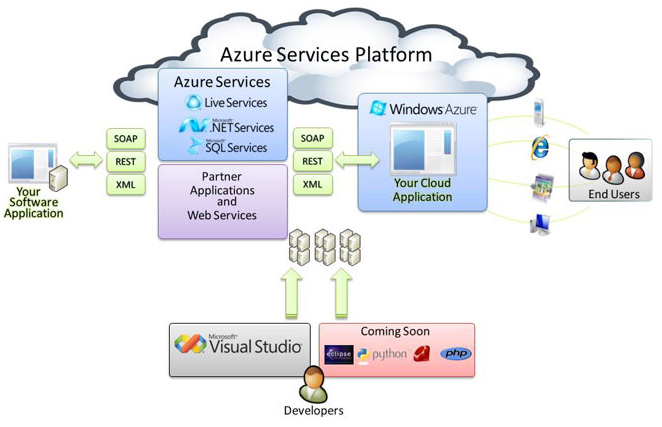
\includegraphics[scale=0.8]{figs/Azure.png} \\
\texttt{High level architectural outline of the Azure cloud}\ftAimg\ftAimgText
\end{center}

Windows Azure is an OS that facilitates both application hosting and data storage. It is upon these two services that users will build and maintain their products once an Azure subscription has been purchased. SQL Azure is a scaled, cloud based implementation of Microsoft SQL Server -- a relational database server and Windows Azure AppFabric represents a collection of cloud computing services at the middleware level.

\section{Available Services}
Notable services are included within AppFabric include, but are not limited to\ftAtwo:\ftAtwoText
\begin{itemize}
\item Access Control Service -- Controls user authorisation on related services and applications.
\item Service Bus -- Ensuring that secure connections are in place on cloud-based applications.
\item Caching -- Allows applications to utilise the high-speed caching service provided by the Microsoft cloud; ensuring a high access time to application data.
\end{itemize}

\section{Cost}
Establishing a competitive price for a cloud-based service is of utmost importance, especially with other notable cloud providers such as Google App Engine and Amazon EC2 in the same consumer space. Microsoft Azure offers three pricing packages\ftAthree{} that are in place for the Azure cloud service. These packages include:\ftAthreeText
\begin{itemize}
\item Consumption-based -- Costs are incurred only when data is used.
\item Subscription-based -- Committing to a fixed price over a specified number of months.
\item Volume-based -- Tailored for large organisations that already possess at least one Microsoft license -- allowing for these services to be integrated into the Microsoft cloud. 
\end{itemize}

\section{Security}

The implementation of rigorous security measures are of critical importance, particularly within a cloud-based service which is available to consumers on a global scale. When users subscribe to the Azure cloud, the credit card used to transfer funds is associated to the user making the payment. In addition, access to the cloud service is performed via signing in through a Windows Live ID account. 

Once a consumer has signed up to the Azure cloud, enforcing a secure means of user authentication is paramount to the security of any stored data. In order to differentiate between application hosting and data storage, Windows Azure uses separate methods used to authenticate users to each service. These methods are outlined in the following table~\cite{AzureSecurity}:

\begin{center}
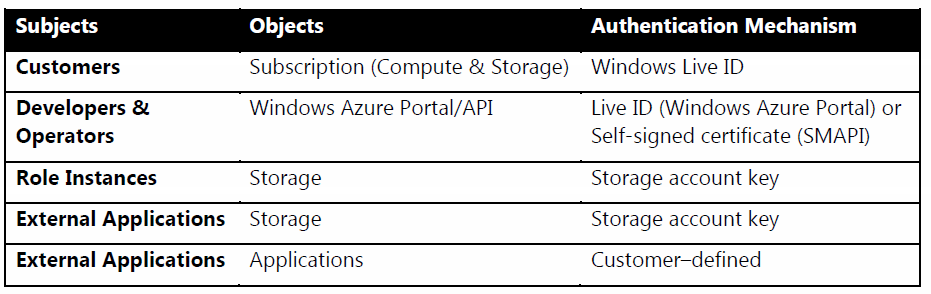
\includegraphics[scale=0.6]{figs/AzureTable.png} \\
\end{center}

Accessing applications hosted on the Azure cloud can be performed by two methods: via the Windows Azure website itself or via the Service Management API (SMAPI). The latter requires the registration of a public/private key and a self-signed certificate associated to each user utilising the cloud service when uploading developed applications. SMAPI authentication references the aforementioned key pair and user certificate before each user session can commence.

When accessing stored content on the Azure cloud, users require an account-specific Storage Account Key (SAK). This key is able to be changed at any time.

The Windows Azure platform must provide fundamental security concepts on its cloud service, in order for consumers to acknowledge that their data is stored safely on the Microsoft cloud. Confidentiality, integrity, availability and accountability are the terms used to describe how security is approached on the Azure platform. Notable features pertaining to each of these terms are as follows~\cite{AzureSecurity}:

\begin{itemize}
\introdef{Confidentiality}{Encryption is used internally within Windows Azure for protecting control channels and is provided optionally for customers who need rigorous data protection capabilities.}

\introdef{Integrity}{Each Virtual Machine (VM) is connected to three local Virtual Hard Drives (VHD). The first VHD contains one of several versions of the Guest OS. The consumer selects the new patches they wish to apply, ensuring that the OS is always at the most recent version. The second VHD contains an image constructed by the Fabric Controller (FC). The last VHD contains configuration data, all paging files and storage.}

\introdef{Availability}{The Azure platform ensures that stored data will not be compromised by employing rigorous backup techniques. These techniques include Data replication and Geo-replication\ftAfour.}\ftAfourText

\clearpage % Ensures next sentence not broken up over pagebreak.
\begin{itemize}
\item Data replication involves replicating the data three times in the same data centre as a precaution against hardware failure – in turn ensuring that data is always available. 

\item Geo-replication involves replicating data between data centres that are not situated within geographic vicinity. This approach safeguards against any natural disasters.
\end{itemize}
\end{itemize}


Adopting the Microsoft Windows Azure software is a viable solution for both a personal or business need to utilise a distributed cloud computing service to store and maintain developed applications. As with moving towards any new software, it is up to the consumer to adequately research many factors such as cost, security, data storage capabilities and data availability when making use of a cloud based hosting service. The consumption and subscription based pricing packages are ideal for consumers who are both unsure of how much data they will need and consumers who wish to move to the Microsoft cloud for a defined month period.
